\documentclass{beamer}
%
% Choose how your presentation looks.
%
% For more themes, color themes and font themes, see:
% http://deic.uab.es/~iblanes/beamer_gallery/index_by_theme.html
%
\mode<presentation>
{
  \usetheme{default}      % or try Darmstadt, Madrid, Warsaw, ...
  \usecolortheme{default} % or try albatross, beaver, crane, ...
  \usefonttheme{default}  % or try serif, structurebold, ...
  \setbeamertemplate{navigation symbols}{}
  \setbeamertemplate{caption}[numbered]
} 

%% \usepackage[english]{babel}
\usepackage[utf8x]{inputenc}
\usepackage{color}
%% \usepackage{listings}
\usepackage{verbatim}

\usepackage[style=british]{csquotes}


%% Presentation title and names of the organization
\title{Email Self-defense \\ Workshop}
%% \author{}
\institute{Free Software Foundation}
% \date{29 Apr 2018}

\begin{document}

\begin{frame}  
  \titlepage
\end{frame}

%% Uncomment these lines for an automatically generated outline.
%% \begin{frame}{Outline}
%%  \tableofcontents
%% \end{frame}

%% Relevance of the email surveillance.
\begin{frame}{Introduction}

\end{frame}

% People use local and global email. Sometimes they must send important private data
% The information can be revealed or intercepted (make an accent on this, maybe a gif demonstration)
\begin{frame}{Surveillance}
  \enquote{If we do nothing, new technologies will give the government new automatic surveillance capabilities that Stalin could never have dreamed of. The only way to hold the line on privacy in the information age is strong cryptography.}
  %% 
  \begin{flushright}
    Phill Zimmerman (1991)
  \end{flushright}

  \begin{center}
    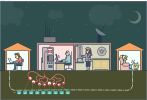
\includegraphics[width=0.8\textwidth]{img/surveillance.pdf}
  \end{center}

\end{frame}

%% Examples of interception by intelligence agencies
\begin{frame}{Government Surveillance}

  \begin{itemize}
  \item PRISM
  \item XKeyscore
  \item Tempora
  \end{itemize}

  \enquote{I don't want to live in a world where everything that I say, everything I do, everyone I talk to, every expression of creativity or love or friendship is recorded. }
  %% 
  \begin{flushright}
    Edward Snowden (2013)
  \end{flushright}
  
\end{frame}

%% Examples of interception by third parties
\begin{frame}{Corporate Surveillance}
  \begin{itemize}
  \item Google profiles people for advertising based on email content
  \item Microsoft Outlook servers automatically access every link present in the email
  \item Facebook profiles users according to the exchanged messages
  \item \dots
  \end{itemize}
  % add references
\end{frame}

%% Examples of sending letters to unverified identities

%% Identify the problem: we should be able to make data available only for target persons and we should be able to verify their identities
%% Thus, we need an encryption and signature

%% Introducing GnuPG
\begin{frame}{Meet GnuPG}
  \begin{minipage}{0.69\linewidth}

    \begin{itemize}
    \item Free software application
    \item Creates public and private digital keys
    \end{itemize}
  \end{minipage}
%
  \begin{minipage}{0.29\linewidth}
    
\includegraphics[width=1.0\textwidth]{img/gnupg.pdf}
  \end{minipage}
  
\end{frame}

%% Principles of working
\begin{frame}{Encryption}
  \begin{minipage}{0.69\linewidth}
    Public key
    \begin{itemize}
    \item Not similar to physical key
    \item Shared other people
    \item Serves for encryption for the specific recipient
    \end{itemize}
  \end{minipage}
%
  \begin{minipage}{0.29\linewidth}
    
\includegraphics[width=1.0\textwidth]{img/encryption.pdf}
  \end{minipage}
\end{frame}

%% Principles of working
\begin{frame}{Decryption}
  \begin{minipage}{0.69\linewidth}
    Private key
    \begin{itemize}
    \item More similar to physical keys
    \item Kept secret on users computer
    \item Serves to open encrypted emails addressed to you
    \item Can be used to create digital signature to proof your authorship of an email
    \end{itemize}
  \end{minipage}
%
  \begin{minipage}{0.29\linewidth}
    
\includegraphics[width=1.0\textwidth]{img/decryption.pdf}
  \end{minipage}
\end{frame}

%% The information is secured now (maybe another gif example)
\begin{frame}
  \begin{center}
    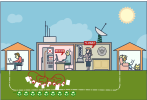
\includegraphics[width=0.8\textwidth]{img/defense.pdf}
  \end{center}

\end{frame}

%% Start of a practical part (instruction, guide etc.)
\begin{frame}{Get the Pieces}
  \begin{itemize}
  \item email client -- IceDove (Thunderbird)
  \item Enigmail plugin
  \end{itemize}
\end{frame}

\begin{frame}{Make Your Keys}
  \begin{itemize}
  \item make a keypair
  \item upload your public key to a keyserver
  \end{itemize}
\end{frame}

\begin{frame}{Try it out}
  \begin{itemize}
  \item Send your public key
  \item Send a test encrypted email
  \item Receive a response
  \item Send a test signed email
  \item Receive a signed response
  \end{itemize}
\end{frame}

\begin{frame}{Learn the Web of Trust}
  \begin{itemize}
  \item Sign a key (check the fingerprint)
  \item If signing a key of a stranger, check their ID
  \item Set ownvertrust
  \end{itemize}
\end{frame}

\begin{frame}{Use it Well}
  \begin{itemize}
  \item When to encrypt
  \item Be wary of invalid keys
  \item Back up your revocation certificate to somewhere safe
  \item Revoke your keys, if someone gets it
  \end{itemize}
\end{frame}

% Free software -- why it is important for privacy
\begin{frame}{Free Software}
  A program is free software if the program's users have four essential freedoms:
  \begin{itemize}
  \item Run the program as you wish
  \item Study how the program works in a source-code form
  \item Help others by distributing exact copies of the program
  \item Contribute to your community by distributing your modified versions
  \end{itemize}

  \enquote{ With software there are just two possibilities; either the user controls the program or the program controls the users.}
  \begin{flushright}
    Richard Stallman
  \end{flushright}

  Proprietary software is fundamentally insecure because its code is hidden from the users.
\end{frame}

\begin{frame}{Further Reading}

  Email Self-defense website,
  \url{emailselfdefense.fsf.org}

  Phil Zimmerman (1991), \emph{Why I Wrote PGP}\\
  \url{www.philzimmermann.com/EN/essays/WhyIWrotePGP.html}

  Surveillance Self-defense,
  \url{ssd.eff.org}

  \url{prism-break.org}

\end{frame}


\begin{frame}

  \begin{center}
    
\includegraphics[width=0.3\textwidth]{img/thanks.pdf}

    \Huge{Thank you!}
  \end{center}
\end{frame}


\end{document}
